\index{general}{BDM element}
\begin{flushright} {\tiny {\color{gray} \tt  pair\_bdm.tex}} \end{flushright}
%~~~~~~~~~~~~~~~~~~~~~~~~~~~~~~~~~~~~~~~~~~~~~~~~~~~~~~~~~~~~~~~~~~~~~~~~~~~~~~~~~~~~~~~~~~~~~~~~~~

This element is mentioned in Kanschat book \cite{kanschat}, section 4.2.14. 
It also exists for quads see section 4.2.39 in the same book.
It is mentioned in \textcite{chen93a} (1993), also check the book by \textcite{brfo}.
It is well described in \textcite{kanschat17}.
There is an entire chapter (14) of \textcite{ergu21_72} dedicated to H(div) and 
section 14.5.1 to BDM elements. 
Check section 4.1.1 of \cite{aubb17} for triangles and quads.

\begin{center}
\url{https://defelement.com/elements/brezzi-douglas-marini.html}
\end{center}

\begin{itemize}
%++++++++++++++++++++++++++++++++++++++++++++++
\item In \textcite{lomw12} we read:

The Brezzi-Douglas-Marini element was introduced by Brezzi, Douglas and Marini in two dimensions 
(for triangles) in \textcite{brdm85} (1985). The element can be viewed as an alternative to the
Raviart-Thomas element using a complete polynomial space. It was later extended to three 
dimensions (tetrahedra, prisms and cubes) in \textcite{nede86} (1986) 
and \textcite{brdd87} (1987). The definition given
here is based on that of \textcite{nede86} (1986).

The Brezzi-Douglas-Marini element was introduced for mixed formulations of second-order elliptic 
equations. However, it is also useful for weakly symmetric discretizations of the elastic stress
tensor; see Farhloul and Fortin (1997); Arnold et al. (2007).

\begin{center}
\includegraphics[width=8cm]{images/pair_bdm/bdm_lomw12}\\
{\captionfont Taken from \cite{lomw12}. }
\end{center}

The dimension of $BDM_q$ is $(q+1)(q+2)$ for a triangle and $\frac12(q+1)(q+2)(q+3)$
for a tetrahedron.

Check book for definition.

A slight modification of the Brezzi-Douglas-Marini element constrains the element space ${\cal V}$ by
only allowing normal components on the boundary of polynomial degree $q-1$ (rather than the full
polynomial degree $q$). Such an element was suggested on rectangles by \textcite{brdf87} (1987), and the
triangular analogue was given in \textcite{brfo}. In similar spirit, elements with differing
degrees on the boundary suitable for varying the polynomial degree between triangles were derived
in \textcite{brdm85b} (1985).

%++++++++++++++++++++++++++++++++++++++++++++++
\item On the defelement website\footnote{\url{https://defelement.org/elements/brezzi-douglas-marini.html}}
we find a lot of information. Note that the mapping is set to 'contravariant Piola'. 
\todo[inline]{I still need to understand and write about this!}
It belongs to the categories 'Vector-valued elements', and 'H(div) conforming elements'

\begin{center}
% -------------------------------------------------------
% This plot is from DefElement (https://defelement.org)
% and is available under a Creative Commons Attribution
% 4.0 International (CC BY 4.0) license:
% https://creativecommons.org/licenses/by/4.0/
% -------------------------------------------------------
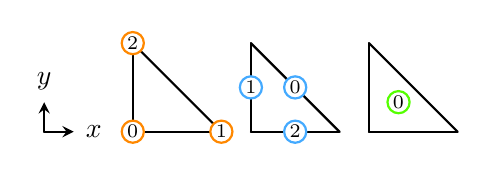
\begin{tikzpicture}[x=1cm,y=1cm]
\definecolor{customcolor0}{HTML}{000000}
\definecolor{customcolor1}{HTML}{44AAFF}
\definecolor{customcolor2}{HTML}{AAAAAA}
\definecolor{customcolor3}{HTML}{DD2299}
\definecolor{customcolor4}{HTML}{FFFFFF}
\definecolor{customcolor5}{HTML}{FF8800}
\definecolor{customcolor6}{HTML}{55FF00}
\draw[-stealth,customcolor0,line width=0.8pt,line cap=round] (25.0,25.0) -- (25.375,25.0);
\draw[-stealth,customcolor0,line width=0.8pt,line cap=round] (25.0,25.0) -- (25.0,25.375);
\node[customcolor0,anchor=west] at (25.405,25.0) {$x$};\node[customcolor0,anchor=south] at (25.0,25.405) {$y$};\draw[customcolor0,line width=0.8pt,line cap=round] (27.25,25.0) -- (26.125,26.125);
\draw[customcolor0,line width=0.8pt,line cap=round] (26.125,25.0) -- (26.125,26.125);
\draw[customcolor0,line width=0.8pt,line cap=round] (26.125,25.0) -- (27.25,25.0);
\draw[customcolor5,line width=0.8pt,fill=customcolor4] (26.125,25.0) circle (4.0pt);
\node[customcolor0,anchor=center] at (26.125,25.0) {\scriptsize 0};\draw[customcolor5,line width=0.8pt,fill=customcolor4] (27.25,25.0) circle (4.0pt);
\node[customcolor0,anchor=center] at (27.25,25.0) {\scriptsize 1};\draw[customcolor5,line width=0.8pt,fill=customcolor4] (26.125,26.125) circle (4.0pt);
\node[customcolor0,anchor=center] at (26.125,26.125) {\scriptsize 2};\draw[customcolor0,line width=0.8pt,line cap=round] (28.75,25.0) -- (27.625,26.125);
\draw[customcolor1,line width=0.8pt,fill=customcolor4] (28.1875,25.5625) circle (4.0pt);
\node[customcolor0,anchor=center] at (28.1875,25.5625) {\scriptsize 0};\draw[customcolor0,line width=0.8pt,line cap=round] (27.625,25.0) -- (27.625,26.125);
\draw[customcolor1,line width=0.8pt,fill=customcolor4] (27.625,25.5625) circle (4.0pt);
\node[customcolor0,anchor=center] at (27.625,25.5625) {\scriptsize 1};\draw[customcolor0,line width=0.8pt,line cap=round] (27.625,25.0) -- (28.75,25.0);
\draw[customcolor1,line width=0.8pt,fill=customcolor4] (28.1875,25.0) circle (4.0pt);
\node[customcolor0,anchor=center] at (28.1875,25.0) {\scriptsize 2};\draw[customcolor6,line width=0.8pt,fill=customcolor4] (29.5,25.375) circle (4.0pt);
\node[customcolor0,anchor=center] at (29.5,25.375) {\scriptsize 0};\draw[customcolor0,line width=0.8pt,line cap=round] (30.25,25.0) -- (29.125,26.125);
\draw[customcolor0,line width=0.8pt,line cap=round] (29.125,25.0) -- (29.125,26.125);
\draw[customcolor0,line width=0.8pt,line cap=round] (29.125,25.0) -- (30.25,25.0);
\end{tikzpicture}
\\
{\captionfont Taken from DefElement \url{https://defelement.org/img/ref-triangle.html}. I have altered 
the font size. Orange: nodes; Blue: edges.}
\end{center}


I reproduce below the figures and basis functions pertaining to the Degree 1 triangle, 
but the site also shows Degree 2 triangle, Degree 1 \& 2 tetrahedron, and so-called 
Lagrange variants.

\begin{center}
\includegraphics[width=3cm]{images/pair_bdm/element-Brezzi-Douglas-Marini-variant-equispaced-triangle-1-dofs}
\includegraphics[width=3cm]{images/pair_bdm/element-Brezzi-Douglas-Marini-variant-equispaced-triangle-1-0}
\includegraphics[width=3cm]{images/pair_bdm/element-Brezzi-Douglas-Marini-variant-equispaced-triangle-1-1}
\includegraphics[width=3cm]{images/pair_bdm/element-Brezzi-Douglas-Marini-variant-equispaced-triangle-1-2}\\
\includegraphics[width=3cm]{images/pair_bdm/element-Brezzi-Douglas-Marini-variant-equispaced-triangle-1-3}
\includegraphics[width=3cm]{images/pair_bdm/element-Brezzi-Douglas-Marini-variant-equispaced-triangle-1-4}
\includegraphics[width=3cm]{images/pair_bdm/element-Brezzi-Douglas-Marini-variant-equispaced-triangle-1-5}\\
{\captionfont Pink: degrees of freedom.}
\end{center}


${\cal V}$ is spanned by 
\[
\left(\begin{array}{c}
1 \\ 0
\end{array}\right),
\left(\begin{array}{c}
0 \\ 1
\end{array}\right),
\left(\begin{array}{c}
x \\ 0
\end{array}\right),
\left(\begin{array}{c}
0 \\ x
\end{array}\right),
\left(\begin{array}{c}
y \\ 0
\end{array}\right),
\left(\begin{array}{c}
0 \\ y
\end{array}\right)
\]
with 
\begin{itemize}
\item DOF \#0 is associated with edge 0 of the reference element with $\vec{\bN}_0$ basis function.
\item DOF \#1 is associated with edge 0 of the reference element with $\vec{\bN}_1$ basis function.
\item DOF \#2 is associated with edge 1 of the reference element with $\vec{\bN}_2$ basis function.
\item DOF \#3 is associated with edge 1 of the reference element with $\vec{\bN}_3$ basis function.
\item DOF \#4 is associated with edge 2 of the reference element with $\vec{\bN}_4$ basis function.
\item DOF \#5 is associated with edge 2 of the reference element with $\vec{\bN}_5$ basis function.
\end{itemize}
and
\begin{eqnarray}
\vec{\bN}_0 &=&  \left(\begin{array}{c} -4x \\ 2y        \end{array}\right) \nn\\  
\vec{\bN}_1 &=&  \left(\begin{array}{c} 2x \\ -4y        \end{array}\right) \nn\\  
\vec{\bN}_2 &=&  \left(\begin{array}{c} 4x+6y-4 \\ -2y   \end{array}\right) \nn\\  
\vec{\bN}_3 &=&  \left(\begin{array}{c} -2x-6y+2 \\ 4y   \end{array}\right) \nn\\  
\vec{\bN}_4 &=&  \left(\begin{array}{c} 2x \\ -6x-4y+4   \end{array}\right) \nn\\  
\vec{\bN}_5 &=&  \left(\begin{array}{c} -4x \\ 6x +2y -2 \end{array}\right) \nn
\end{eqnarray}

 

















\end{itemize}

